% !TeX spellcheck = ru_RU_yo
% !TEX program = xelatex

\documentclass[pta]{build/scs-iam}

\usepackage[justification=centering]{caption} 
\captionsetup[table]{skip=15pt}
\captionsetup[table]{justification=centering}

\begin{document}
  \pagestyle{headcenter}

  \newgeometry{
  top=20mm,
  right=15mm,
  bottom=20mm,
  left=20mm,
  bindingoffset=0cm
}

\thispagestyle{empty}

\begin{center}
  {
    \bfseries
    {
      \subnormal
      Министерство науки и высшего образования Российской Федерации
    } \\[-0.5em]
    {
      \scriptsize
      ФЕДЕРАЛЬНОЕ ГОСУДАРСТВЕННОЕ АВТОНОМНОЕ ОБРАЗОВАТЕЛЬНОЕ УЧРЕЖДЕНИЕ ВЫСШЕГО ОБРАЗОВАНИЯ
    } \\[-0.25em]
    {
      \subnormal
      “САНКТ-ПЕТЕРБУРГСКИЙ НАЦИОНАЛЬНЫЙ ИССЛЕДОВАТЕЛЬСКИЙ \\[-0.5em]
      УНИВЕРСИТЕТ ИНФОРМАЦИОННЫХ ТЕХНОЛОГИЙ, \\[-0.75em]
      МЕХАНИКИ И ОПТИКИ”
    } \\[3.25em]
    {
      \normalsize
      ВЫПУСКНАЯ КВАЛИФИКАЦИОННАЯ РАБОТА
    } \\[3.75em]
    {
      \normalsize
      <<РАЗРАБОТКА ПРОГРАММЫ ПОИСКА АНАЛОГОВ\\[-0.5em]
      НА ОСНОВЕ МАШИННОГО ОБУЧЕНИЯ>>
    } \\[5.75em]
  }
\end{center}

\begin{flushright}
  {
    \small
    \begin{minipage}{.7\textwidth}
      \titledline{Автор}\addsignatureskip
      \hspace{-5pt}$\underset{\text{\scriptsize (Фамилия, Имя, Отчество)}}{\underline{\makebox[\remaining][s]{\strut\hfill Канукова Софья Алановна\hfill}}}$
      \hfill
      \signature \\[-0.5em]

      \titledline{Направление подготовки (специальность)}
      $\underset{\text{\scriptsize (код, наименование)}}{\underline{\makebox[\remaining][s]{\strut\hfill 09.03.01 --\hfill}}}$ \\[-0.5em]
      $\underline{\makebox[\textwidth][s]{\strut\hfill Информатика и вычислительная техника\hfill}}$ \\[-0.5em]

      \titledline{Квалификация}
      $\underset{\text{\scriptsize (бакалавр, магистр)}}{\underline{\makebox[\remaining][s]{\strut\hfill бакалавр\hfill}}}$ \\[-0.5em]

      \titledline{Руководитель ВКР}\addsignatureskip
      \hspace{-5pt}$\underset{\text{\scriptsize (Фамилия, И., О.,  ученое звание, степень)}}{\underline{\makebox[\remaining][s]{\strut\hfill Тропченко А. А., к.т.н., доцент\hfill}}}$
      \hfill\signature \\[3em]

      \textbf{К защите допустить} \\[0.25em]
      \titledline{Руководитель ОП}\addsignatureskip
      \hspace{-5pt}$\underset{\text{(Фамилия, И., О.,  ученое звание, степень)}}{\underline{\makebox[\remaining][s]{\strut\hfill Алиев Т. И., д.т.н., профессор\hfill}}}$
      \hfill\signature \\[-0.25em]

      \hfill\datetemplate
    \end{minipage}
  }
\end{flushright}

\vfill

\begin{center}
  {
    \normalsize
    Санкт-Петербург, 2019 г.
  }
\end{center}

\restoregeometry

\clearpage

\newgeometry{
  top=20mm,
  right=20mm,
  bottom=20mm,
  left=15mm,
  bindingoffset=0cm
}

\thispagestyle{empty}

{
  \small
  \parindent0pt

  Студент
  $\underset{\text{\scriptsize (Фамилия, Имя, Отчество)}}{\underline{\text{\strut ~Канукова Софья Алановна~}}}$
  \hfill
  Группа
  $\underline{\text{\strut ~P3402~}}$
  \hfill
  Факультет
  $\underline{\text{\strut ~ПИиКТ~}}$ \\[-0.5em]

  \titledline{Направленность (профиль), специализация}
  $\underline{\makebox[\remaining][s]{\strut\hfill \hfill}}$
  $\underline{\makebox[\textwidth][s]{\strut\hfill Вычислительные машины, комплексы, системы и сети \hfill}}$ \\[0.25em]

  ВКР принята \datetemplate \\[-1em]

  Оригинальность ВКР $\underline{\makebox[7em][s]{\strut}}$\,\% \\[-1em]

  ВКР выполнена с оценкой $\underline{\makebox[12em][s]{\strut}}$ \\[-1em]

  Дата защиты \datetemplate \\[-1em]

  \titledline{Секретарь ГЭК}\addsignatureskip
  \hspace{-5pt}$\underset{\text{\scriptsize (Фамилия, И., О.)}}{\underline{\makebox[\remaining][s]{\strut}}}$
  \hfill\signature \\[0.25em]

  Листов хранения $\underline{\makebox[12em][s]{\strut}}$ \\[-1em]

  Демонстрационных материалов/Чертежей хранения $\underline{\makebox[12em][s]{\strut}}$
}

\restoregeometry

\clearpage

  \newgeometry{
  top=20mm,
  right=15mm,
  bottom=20mm,
  left=20mm,
  bindingoffset=0cm
}

\thispagestyle{empty}

\begin{center}
  {
    \bfseries
    {
      \subnormal
      Министерство науки и высшего образования Российской Федерации
    } \\[-0.5em]
    {
      \scriptsize
      ФЕДЕРАЛЬНОЕ ГОСУДАРСТВЕННОЕ АВТОНОМНОЕ ОБРАЗОВАТЕЛЬНОЕ УЧРЕЖДЕНИЕ ВЫСШЕГО ОБРАЗОВАНИЯ
    } \\[-0.25em]
    {
      \subnormal
      “САНКТ-ПЕТЕРБУРГСКИЙ НАЦИОНАЛЬНЫЙ ИССЛЕДОВАТЕЛЬСКИЙ \\[-0.5em]
      УНИВЕРСИТЕТ ИНФОРМАЦИОННЫХ ТЕХНОЛОГИЙ, \\[-0.75em]
      МЕХАНИКИ И ОПТИКИ” \\[2em]
    }
  }
\end{center}

\small

\begin{flushright}
  \begin{minipage}{.5\textwidth}
    {
      \hfill\textbf{УТВЕРЖДАЮ}\hfill
    }

    \titledline{Руководитель ОП}

    \setlength{\remaining}{\textwidth}\addsignatureskip
    $\underset{\text{\scriptsize (Фамилия, И.О.)}}{\underline{\makebox[\remaining][s]{\strut\hfill}}}$
    \hfill\signature \\[-0.5em]

    \hfill\datetemplate \\[0.35em]
  \end{minipage}
\end{flushright}

\begin{center}
  {
    \bfseries
    {
      \normalsize
      З А Д А Н И Е \\
    }
    НА  ВЫПУСКНУЮ  КВАЛИФИКАЦИОННУЮ  РАБОТУ \\[1.5em]
  }
\end{center}

{
  \parindent0pt

  \textbf{Студенту}
  $\underline{\text{\strut Кануковой С. А.~~}}$
  \hfill
  \textbf{Группа}
  $\underline{\text{\strut P3402~~}}$
  \hfill
  \textbf{Факультет}
  $\underline{\text{\strut ПИиКТ~~}}$ \\[-0.5em]

  \titledline{\textbf{Руководитель ВКР}}
  $\underset{
    \text{\scriptsize (ФИО, ученое звание, степень, место работы, должность)}
  }{
    \underline{\makebox[\remaining][s]{\strut Тропченко Андрей Александрович, к.т.н., доцент, Университет ИТМО\hfill}}
  }$ \\[-0.5em]

  \textbf{1 Наименование темы}
  \uline{Разработка программы поиска аналогов на основе машинного обучения\hfill} \\[-1em]
  
  \titledline{\textbf{Направление подготовки (специальность)}}
  $\underline{
    \makebox[\remaining][s]{\strut 09.03.01 -- Информатика и вычислительная техника\hfill}
  }$ \\[-1em]

  \titledline{\textbf{Направленность (профиль)}}
  $\underline{
    \makebox[\remaining][s]{\strut Вычислительные машины, комплексы, системы и сети\hfill}
  }$ \\[-1em]

  \titledline{\textbf{Квалификация}}
  $\underline{
    \makebox[\remaining][s]{\strut бакалавр\hfill}
  }$ \\[-1em]

  \textbf{2 Срок сдачи студентом законченной работы}\hfill\datetemplate \\[-1em]

  \textbf{3 Техническое задание и исходные данные к работе} \\
  \uline{
    Разработать программу поиска аналогов, провести тестирование и апробацию.\hfill
  }\\
  \uline{
    Исходные данные:\hfill
  }\\
  \uline{
    - набор данных для обучения модели\hfill
  }\\
  \uline{
  Требования к программе:\hfill
  }\\
  \uline{
  - результат поиска с точностью выше 90\%\hfill
  }\\
  \uline{
  - программа не должна находить аналоги, которые не содержат ключевые слова (идентификацион-\hfill
  }\\
   \uline{
   ный номер, название модели), указанные при поиске\hfill
  }\\[-1em]
}

\restoregeometry

\clearpage

\newgeometry{
  top=20mm,
  right=20mm,
  bottom=20mm,
  left=15mm,
  bindingoffset=0cm
}

\thispagestyle{empty}

{
  \parindent0pt

  \textbf{4 Содержание выпускной квалификационной работы (перечень подлежащих разработке} \\
  \textbf{вопросов)}\\
  \uline{
    4.1 Обзор предметной области;\hfill
  }\\
  \uline{
    4.2 Выбор инструментов разработки;\hfill
  }\\
  \uline{
    4.3 Описание процесса разработки;\hfill
  }\\
  \uline{
    4.4 Апробация результатов разработки.\hfill
  }\\[-1em]

  \textbf{5 Перечень графического материала (с указанием обязательного материала)} \\
  \uline{
    Презентация по проделанной работе (в формате PDF)\hfill
  }\\
  \uline{
    Слайд №1 "Постановка задачи"\hfill
  }\\
  \uline{
    Слайд №2 "Архитектура программы"\hfill
  }\\
  \uline{
    Слайд №3 "Характеристики программы"\hfill
  }\\
  \uline{
    Слайд №4 "Примеры работы программы"\hfill
  }\\[-1em]

  \textbf{6 Исходные материалы и пособия} \\
  \uline{
    6.1 Флах, Петер Машинное обучение. Наука и искусство построения алгоритмов, которые извлека-\hfill
  }\\
  \uline{
    ют знания из данных. Учебник // Петер Флах. - М.: ДМК Пресс. 2015.\hfill
  }\\
  \uline{
    6.2 Батура Т.В. Методы автоматической классификации текстов // Программные продукты и системы. 2017. №1. - Режим доступа: https://cyberleninka.ru/article/n/metody-avtomaticheskoy-klassifikatsii-\hfill
  }\\
  \uline{
    tekstov\hfill
  }\\
  \uline{
    6.3 Scikit-learn Documentation [Электронный ресурс] // Официальный сайт проекта Scikit-learn. 2007-2019. - Режим доступа: https://scikit-learn.org/stable/documentation.html\hfill
  }\\[-1em]

  \textbf{7 Дата выдачи задания} \datetemplate\\[-1em]

  Руководитель ВКР~~\signature\\[-1em]

  Задание принял к исполнению~~\signature\hfill\datetemplate\\
}

\normalsize
\restoregeometry

\clearpage

  \newgeometry{
  top=20mm,
  right=15mm,
  bottom=20mm,
  left=20mm,
  bindingoffset=0cm
}

\thispagestyle{empty}

\begin{center}
  {
    \bfseries
    {
      \subnormal
      Министерство образования и науки Российской Федерации
    } \\[-0.5em]
    {
      \scriptsize
      ФЕДЕРАЛЬНОЕ ГОСУДАРСТВЕННОЕ АВТОНОМНОЕ ОБРАЗОВАТЕЛЬНОЕ УЧРЕЖДЕНИЕ ВЫСШЕГО ОБРАЗОВАНИЯ
    } \\[-0.25em]
    {
      \subnormal
      “САНКТ-ПЕТЕРБУРГСКИЙ НАЦИОНАЛЬНЫЙ ИССЛЕДОВАТЕЛЬСКИЙ \\[-0.5em]
      УНИВЕРСИТЕТ ИНФОРМАЦИОННЫХ ТЕХНОЛОГИЙ, \\[-0.75em]
      МЕХАНИКИ И ОПТИКИ”
    }
  }
\end{center}

\small

\begin{center}
  \vskip -1em
  {
    \bfseries
    {
      \large
      АННОТАЦИЯ \\
    }
    ВЫПУСКНОЙ  КВАЛИФИКАЦИОННОЙ  РАБОТЫ \\[1.5em]
  }
\end{center}

{
  \parindent0pt

  \titledline{\textbf{Студент}}
  $\underset{
    \text{\scriptsize (Фамилия, Имя, Отчество)}
  }{
    \underline{\makebox[\remaining][s]{~Яшин Александр Павлович\hfill}}
  }$ \\[-0.5em]

  \textbf{Наименование темы ВКР}
  \uline{~Разработка системы сборки Embedded Linux \hfill} \\[-1em]

  \textbf{Наименование организации, где выполнена ВКР}
  \uline{~Университет ИТМО\hfill} \\[-1.75em]
}

\begin{center}
  \textbf{ХАРАКТЕРИСТИКА ВЫПУСКНОЙ КВАЛИФИКАЦИОННОЙ РАБОТЫ}
\end{center}

\vskip -1em

{
  \parindent0pt

  \textbf{1 Цель исследования}
  \uline{Создание веб-приложения для обеспечения взаимодействия пользователя с~программным пакетом RTKLIB, используемым во~встраиваемом решении, с~помощью кроссплат\-форменного графического интерфейса\hfill} \\[-1em]

  \textbf{2 Задачи, решаемые в ВКР} \\
  \uline{
    2.1 Изучение состава и~возможностей программного комплекса RTKLIB;\hfill
  }\\
  \uline{
    2.2 Анализ существующих веб-приложений, предназначенных для работы устройствами, у~кото\-рых отсутствую органы управления;\hfill
  }\\
  \uline{
    2.3 Проектирование и~разработка приложения;\hfill
  }\\
  \uline{
    2.4 Тестирование и~апробация разработанного приложения.\hfill
  }\\[-1em]

  \textbf{3 Число источников, использованных при составлении обзора}
  \uline{\hfill 8\hfill} \\[-1em]

  \textbf{4 Полное число источников, использованных в работе}
  \uline{\hfill 38\hfill} \\[-1em]

  \textbf{5 В том числе источников по годам}
  \begin{figure}[h!]
    \centering
    \begin{tabular}{| *{6}{>{\centering\small\vspace{2pt}}m{2cm} |}}
      \toprule
      \multicolumn{3}{|>{\bfseries\small}c|}{Отечественных} & \multicolumn{3}{>{\bfseries\small}c|}{Иностранных} \tabularnewline
      \midrule
      Последние 5 лет & От 5 до 10 лет & Более 10 лет & Последние 5 лет & От 5 до 10 лет & Более 10 лет \tabularnewline
      \midrule
      7 & 0 & 0 & 31 & 0 & 0 \tabularnewline
      \bottomrule
    \end{tabular}
  \end{figure}\\[-2.5em]

  \titledline{\textbf{6 Использование информационных ресурсов Internet}}
  $\underset{
    \text{(да, нет, число ссылок в списке литературы)}
  }{
    \underline{\makebox[\remaining][s]{\hfill да, 37 \hfill}}
  }$
}

\restoregeometry

\clearpage

\newgeometry{
  top=20mm,
  right=20mm,
  bottom=20mm,
  left=15mm,
  bindingoffset=0cm
}

\thispagestyle{empty}

{
  \parindent 0pt

  \textbf{7 Использование современных пакетов компьютерных программ и технологий}
  \begin{figure}[h!]
    \centering
    \begin{tabular}{| >{\small\vspace{2pt}}m{10cm} | >{\centering\small\vspace{2pt}}m{3cm} |}
      \toprule
      \centering\textbf{Пакеты компьютерных программ и технологий} & \textbf{Раздел работы} \tabularnewline
      \midrule
      Программный пакет RTKLIB & 1, 2, 3, 4 \tabularnewline
      \midrule
      Язык программирования JavaScript & 3 \tabularnewline
      \midrule
      Менеджер пакетов NPM (Node.js) & 3 \tabularnewline
      \midrule
      Система сборки веб-приложений Webpack & 3 \tabularnewline
      \midrule
      Babel (транспилер) & 3 \tabularnewline
      \bottomrule
    \end{tabular}
  \end{figure}\\[-2.5em]

  \textbf{8 Краткая характеристика полученных результатов}
  \uline{В~результате работы было разработано веб-приложение, позволяющее пользователю взаимодействовать с~программным пакетом RTKLIB, используемым в~ГНСС-модулях и~ГНСС-приёмниках компании Emlid. Разработанное приложение было протестировано и~успешно прошло апробацию у~пользователей.\hfill} \\[-1em]

  \titledline{\textbf{9 Полученные гранты, при выполнении работы}}
  $\underset{
    \text{(название гранта)}
  }{
    \underline{\makebox[\remaining][s]{\hfill нет\hfill}}
  }$ \\[-1em]

  \titledline{\textbf{10 Наличие публикаций и выступлений на конференциях по теме выпускной работы}}
  $\underset{
    \text{(да, нет)}
  }{
    \underline{\makebox[\remaining][s]{\hfill да\hfill}}
  }$ \\[0.5em]
  \titledline{а) 1}
  $\underset{
    \text{(Библиографическое описание публикаций)}
  }{
    \underline{\makebox[\remaining][s]{\hfill}}
  }$ \\[0.5em]
  \titledline{б) 1}
  $\underset{
    \text{(Библиографическое описание выступлений на конференциях)}
  }{
    \underline{\makebox[\remaining][s]{Кузнецов А.А. Разработка веб-приложения для работы с программным пакетом высокоточно-}}
  }$
  \uline{го позиционирования RTKLIB // Конференция: XLVII Научная и учебно-методическая конферен\-ция Университета ИТМО, секция: Итоги выполнения НИР с участием магистрантов и аспирантов, подсекция: Исследование и разработка в области информационных технологий, 2018.\hfill} \\[-3em]
  \begin{flushright}
    2~\,\underline{\makebox[\remaining][s]{Кузнецов А.А. Разработка веб-приложения для работы с программным пакетом высокоточно-}}
  \end{flushright}
  \vskip -0.75em
  \uline{го позиционирования RTKLIB // Конференция: VII Конгресс молодых учёных, секция: Информа\-ционные технологии, 2018.\hfill} \\[-1em]

  Студент
  $\underset{
    \text{\scriptsize (Фамилия, И., О.)}
  }{
    \underline{\makebox[12em][s]{\strut\hfill}}
  }$~~ \signature\\[-0.5em]
  
  Руководитель
  $\underset{
    \text{\scriptsize (Фамилия, И., О.)}
  }{
    \underline{\makebox[12em][s]{\strut\hfill}}
  }$~~ \signature\\[-0.5em]
  
  \datetemplate
}

\normalsize
\restoregeometry

\clearpage


  \setcounter{page}{4}

  \section*{СОДЕРЖАНИЕ}
  \tableofcontents

  \newpage

  \mysection*{ВВЕДЕНИЕ}

\textbf{Актуальность темы}. В конце 20-го века с развитием информационных технологий стало возможным делать покупки не выходя из дома, возможности для этого предоставляют интернет-магазины. С ростом количества интернет-магазинов появились системы мониторинга цен и предложений конкурентов для предпринимателей, владеющих интернет-магазинами. Такой мониторинг позволяет автоматически формировать
цены на товары в магазине в соответствии с текущей ситуацией на рынке. Одной из важнейших задач таких систем является установление связей между товарами предпринимателя и его конкурентов. Автоматизация подобных процессов позволяет людям сэкономить время и ресурсы. 

\textbf{Целью работы} является создание программы поиска аналогов на основе машинного обучения. Такая программа сможет без ручного внесения в базу устанавливать связи между товарами владельца интернет-магазина и его конкурентов. Таким образом, нет необходимости отслеживать появление новых товаров у конкурентов и заносить новую связь в базу, программа найдет соответсвие сама, обучившись на большом наборе подобных связей.

Для достижения цели исследования был сформулирован следующий ряд \textbf{задач}:

\begin{itemize}
  \item провести обзор машинного обучения;
  \item определить требования к программе;
  \item осуществить проектирование и разработку программы;
  \item произвести тестирование приложения.
\end{itemize}

\textbf{Объем и структура работы}. Работа содержит 38 страниц печатного текста, 5 рисунков, 1 таблицу, список литературы, включающий 10 источников. Работа состоит из введения, четырех частей и заключения. Во введении обоснована актуальность работы, определены цель и задачи исследования. В первой части произведено краткое описание области машинного обучения, а также обзор существующих решений. Вторая часть содержит описание структуры программы и выбранных средст разработки. Третья глава описывает реализацию программы. Четвертая глава описывает тестирование разработанной программы и харатеристики работы. В заключении приведены основные результаты работы и возможные направления для дальнейшего развития.

\newpage

  \mysection{АНАЛИЗ ПРЕДМЕТНОЙ ОБЛАСТИ}
\
\subsection{Машинное обучение. Задача классификации}
\

\textbf{Машинное обучение} – группа методов искусственного интеллекта, которые используются компьютерными системами для эффективного выполнения конкретной задачи без использования явных инструкций, вместо этого обучаясь на множестве решений сходных задач.

Машинное обучение подразделяется на обучение по прецедентам, что означает выявление общих закономерностей по частным эмпирическим данным, и дедуктивное обучение, при котором формируется база знаний на основе формализованных знаний экспертов.

В данной работе речь пойдет об обучении по прецедентам, одним из подтипов которого является обучение с учителем. Обучение с учителем – самый распространенный случай, оно производится на наборе обучающих примеров, каждый из которых представлет собой пару "объект, ответ". В процессе обучения выводится функциональная зависимость ответа от объекта и строится алгоритм, который позволяет отображать входные данные в выходные. Когда множество возможных ответов конечно, говорят о задачах классификации и распознавания образов.

\textbf{Задача классификации} – ответ принадлежит конечному множеству, он называется меткой класса. Класс представляет собой множество объектов, которые соответсвуют данному значению метки. Задано конечное множество объектов, для которых известно, к каким классам они относятся. Это множество называется выборкой. Классовая принадлежность остальных объектов неизвестна. Требуется построить алгоритм, способный классифицировать произвольный объект из исходного множества.

  \begin{figure}[h!]
    \centering
    \setlength{\fboxsep}{5pt}
    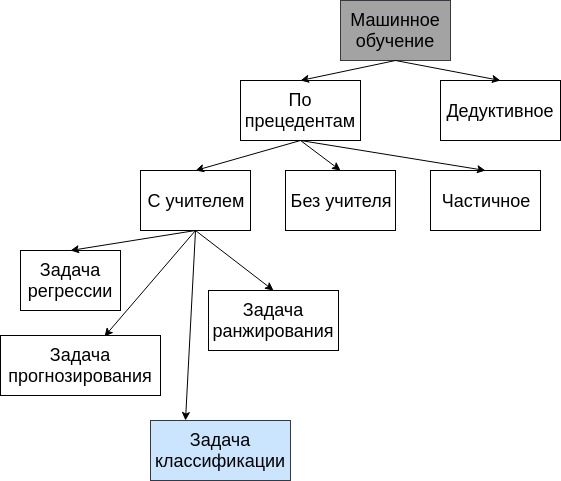
\includegraphics[width=.9\textwidth]{img/ml}
    \vspace*{6pt}
    \caption{Машинное обучение}\label{fig:project-tree}
  \end{figure}

На рисунке 1.1 представлено дерево способов и задач, которые решаются машинным обучением. Дерево неполное, так как существует очень много способов машинного обучения. Поэтому на данном рисунке показана основная ветвь, имеющая прямое отношение к поставленной задаче.

\textbf{Классификатором} называется отображение $\widehat{c}: \mathcal{X} \to \mathcal{C}$, где 
\
$\mathcal{C} = \{C_{1}, C_{2}, \dots, C_{k}\}$ — конечное множество меток классов. Под $C_{i}$ можно также понимать множество объектов, которые относятся к классу с номером $i$. Знак "крышки" означает, что $\widehat{c}(x)$ — оценка истинной, но неизвестной функции $c(x)$. Обучающие примеры для классификатора имеют вид пар $(x,c(x))$, где $x \in \mathcal{X}$ — объект, а $c(x)$ — истинный класс, к которому принадлежит этот объект. Под обучением классификатора понимается выявление функции $\widehat{c}$, которая как можно лучше аппроксимирует $c$ не только на обучающем наборе, но в идеале и на всем пространстве объектов.\cite{MLFLACH}

\textbf{Типы классификации:}
\begin{itemize}
  \item Бинарная классификация – требуется определить к какому из двух классов относится объект, простой в техническом отношении случай, который служит основой для решения более сложных задач;
  \item Многоклассовая классификация – более двух классов, задача классификации становится более трудной, решающая граница не столь очевина, как в первом случае;
  \item Непересекающиеся классы – объект относится только к одному из множества классов;
  \item Пересекающиеся классы – объект может относиться одновременно к нескольким классам;
  \item Нечёткие классы – определяется степень принадлежности объекта каждому из классов.
\end{itemize}

\textbf{Типы входных данных:}
\begin{itemize}
  \item Признаковое описание — каждый объект – это набор признаков, признаки могут быть числовыми или нечисловыми;
  \item Матрица расстояний между объектами. Каждый объект описывается расстояниями до всех остальных объектов обучающей выборки. С этим типом входных данных работают методы ближайших соседей, парзеновского окна, потенциальных функций;
  \item Временной ряд или сигнал представляет собой последовательность измерений во времени;
  \item Изображение или видеоряд.
\end{itemize}

Также входные данные могут представляться в виде графов, текстов. Они приводятся к первому или второму типу путём предварительной обработки данных и извлечения признаков.

Классификация текстов (документов) — одна из задач информационного поиска, заключающаяся в определении принадлежности текста к одному из нескольких классов на основании содержания текста. Классификацию документов можно организовать с помощью методов машинного обучения. При таком подходе сохраняется необходимость разметки обучающего множества, то есть человек заранее связывает некоторые документы с классами, тем самым формируя обучающий корпус. Таким образом, классификация документов является примером обучения с учителем, в роли учителя выступает человек, размечающий тексты. 

\textbf{Этапы обработки:}
\begin{itemize}
  \item Индексация документов. Переход к числовой модели, преобразование документов в вектора и определение весов слов;
  \item Построение и обучение классификатора. Могут использоваться различные методы машинного обучения: решающие деревья, наивный байесовский классификатор, нейронные сети, метод опорных векторов и др.;
  \item Оценка качества классификации.
\end{itemize}

\newpage
\subsection{Подготовка данных и извлечение признаков}
\

В рамках данной работы речь идет о классификации текстов или документов. Документы, которые требуется классифицировать, – названия моделей конкурента, а множество классов – это множество названий моделей владельца магазина. Входные данные в обучающем корпусе являются текстами, которые необходимо преобразовать и представить в виде, в котором на них сможет обучаться выбранная модель. С использованием всех объектов-документов в наборе обучающих данных составляется словарь размера $n$ - множество всех признаков, встретившихся в документах. Процесс выделения из текстов признаков с использованием разделителя называется токенизацией. 

Далее каждый документ представляется вектором размера $n$, в котором каждому признаку из словаря ставится в соответствие количество вхождений данного признака в документ.

После преобразования текстовых документов к векторам происходит переход к частотности. TF (term frequency — частота слова) — отношение числа вхождений некоторого слова к общему числу слов документа. Оценивается важность слова $t_{i}$ в пределах отдельного документа.

\

\large tf$(t, d) = \frac{n_{t}}{\sum_{k}n_{k}}$, \normalsize

\

где $n_{t}$ — число вхождений слова $t$ в документ, а в знаменателе общее количество слов в документе.

\

Еще одно уточнение меры — IDF (inverse document frequency — обратная частота документа) — инверсия частоты, с которой некоторое слово встречается во всех документах корпуса данных. Таким образом, чем чаще слово встречается в пределах всех коллекции, тем меньше становится вес таких слов. Для каждого слова существует только одно IDF в пределах коллекции.

\

\large idf$(t, D) = \log\frac{|\:D\:|}{| \{ \: d_{i} \: \in \: D \: | \: t \in \: d_{i} \: \}| \:}$, \normalsize

\

где $|\:D\:|$ — общее число документов в обучающем корпусе, а в знаменателе логарифма число документов, в которых встречается $t$.

\

\large tf-idf$(t, D) = $tf$(t, d) \times$ idf$(t, D)$, \normalsize

\

Мера TF-IDF это произведение TF и IDF. После нормализации наибольший вес получат слова, которые часто встречаются в пределах какого-либо документа, но редко во всех коллекции документов. 

\newpage
\subsection{Машина опорных векторов}
\

Существует множество алгоритмов, которые используются для обучения текстовых классификаторов. Одним из них является метод опорных векторов, выбранный мной в соответстивии с реультатами исследования, проведенными Т. В. Батурой в статье "Методы автоматической классификации текстов".\cite{TEXTCLASSIFICATION} В этой статье проводится сравнение нескольких алгоритмов и выявляется, что одно из лучших соотношений характеристик качества достигается при использовании метода опорных векторов (для коллекция текстов объемом 1 000–2 000 текстов точность 80–85 \%, полнота 83–87 \%).

\

  \begin{figure}[h!]
    \centering
    \setlength{\fboxsep}{5pt}
    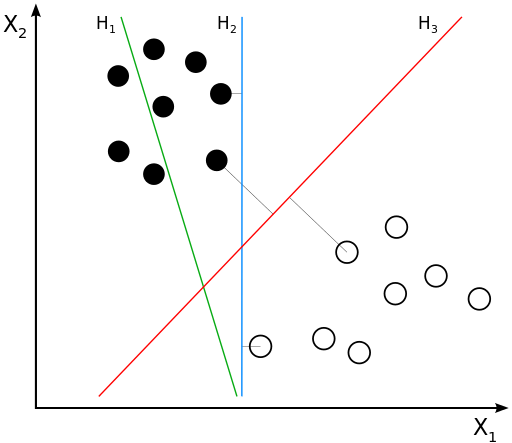
\includegraphics[width=.9\textwidth]{img/svm}
    \vspace*{6pt}
    \caption{Метод опоных векторов}\label{fig:project-tree}
  \end{figure}

\

Машина опорных векторов (метод опорных векторов) – это модель на основе обучения с учителем. Существует множество векторов размера $n$. Каждый из них представляется точкой в $n$-мерном пространстве. Основная задача состоит в том, чтобы найти гиперплоскость размерности $(n-1)$, которая сможет разделить точки в указанном пространстве, тем самым обозначая их принадлежность к разным классам. Причем расстоние от ближайших к гиперплоскости точек до самой гиперплоскости, которое называется зазором, должно быть максимальным, так как предполагается, что это обеспечит наибольшую точность при классификации. В случае линейной неразделимости, то есть когда невозможно найти гиперплоскость, разделяющую множество точек, все вектора переводятся в пространство более высокой размерности и определяется разделяющая гиперплоскость.\cite{Vyugin}

В случае мультиклассовой классификации применяется решающее правило, основанное на разбиении задачи на бинарные по схеме "один против остальных" (one-vs-rest). Обучается n классификаторов, где n – количество классов. Классификатор с самым высоким значением функции выхода используется при классификации.

На рисунке 1.2 показано множество векторов, изображенных в виде точек, и несколько гиперплоскостей, разделяющих эти точки на два класса. Точки, ближайшие к гиперплоскостям, называются опорными векторами. По расстоянию от гиперплоскости до опорных векторов (перпендикуляр изображен серым цветом) определяется величина зазора. На рисунке оптимальной гиперплоскостью является $H_{3}$, так как зазор является максимальным.

\newpage
\subsection{Анализ имеющихся решений}
\

Одним из имеющихся решений является Elasticsearch. \textbf{Elasticsearch} - свободная программная поисковая система, написанная на языке Java, которая используется большим числом крупных сайтов и компаний, например, GitHub, Foursquare, SoundCloud и другие. Данная система может использоваться для решений многих задач, одной из которых является сопоставление товаров для систем мониторинга цен конкурентов.\cite{ELASTIC} Однако для организации связей товаров Elasticsearch требует четкого задания классов синонимов, то есть групп слов, которые будут распознаваться как один и тот же признак в названии товара. Такой способ не подходит, если в поиске участвует большой объем названий товаров из разных категорий и невозможно вручную установить связи между словами из-за их количества и неопределенности.

\newpage
\subsection{Постановка задач исследования}
В рамках данной работы поставлена задача разработать программу, которая сможет находить связи между товарами, основываясь на предсказаниях обученного на корпусе данных классификатора.
Для решения поставленной цели необходимо решить следующие задачи:
\begin{itemize}
  \item Определить требования к программе;
  \item Спроектировать архитектуру программы;
  \item Реализовать программу в соответствии с разработанной архитектурой;
  \item Провеси тестирование.
\end{itemize}
\newpage

  \mysection{РАЗРАБОТКА АРХИТЕКТУРЫ ПРОГРАММЫ}
\
\subsection{Требования к реализуемой программе}
\

Требования к программам и системам можно разделить на функциональные и нефункциональные. Функциональные требования позволяют обозначить функционал, которым должна обладать программа для удовлетворения просьб заказчика. Нефункциональные требования — это дополнительные атрибуты качества, которые важны для разработчика и заказчика.

К разрабатываемой программы были поставлены следующие функциональные требования:

\begin{itemize}
  \item Программа должна иметь функционал для сохранения и загрузки обученной модели;
  \item Программа не должна находить связь, если в запросе был указан товар, который не существует в базе клиента;
  \item Предсказания должны осуществляться с точностью более 90\%;
  \item Время ответа классификатора не должно превышать 0.1 с.
\end{itemize}

\
Нефункциональные требования:
\begin{itemize}
  \item Программа должна иметь API для возможности интеграции в приложение.
\end{itemize}

\newpage

\subsection{Проектирование архитектуры}
\

Для разработки программы была выбрана модульная архитектура. Модульная архитектура — архитектура, при которой программа организована как совокупность независимых друг от друга блоков, структура и поведение которых подчиняются определенным правилам. Использование такой архитектуры позволяет упростить тестирование и масштабирование, так как каждый модуль имеет строго определенные задачи, которые можно дополнять и тестировать отдельно от остальных модулей.

Использование данной архитектуры позволило разбить программу на три фрагмента: обучение, классификация, API. Структура программы представлена на рисунке 2.1.

\


  \begin{figure}[h!]
    \centering
    \setlength{\fboxsep}{5pt}
    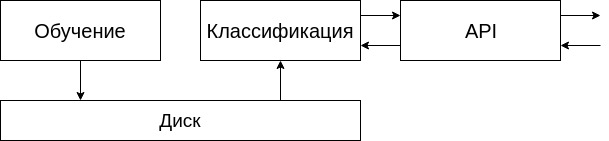
\includegraphics[width=.9\textwidth]{img/module-structure}
    \vspace*{6pt}
    \caption{Структура программы}\label{fig:project-tree}
  \end{figure}


Одной из основных задач разработки является выбор языка программирования. Для реализации программы был выбран Python. Python — высокоуровневый язык программирования общего назначения. Отличительной чертой Python является минималистичность сиктаксиса, что повышает произвоидельность и скорость разработчика, а также читаемость кода.\cite{Python} Простота Python в совокупности с большим количеством библиотек как для работы с данными, так и для машинного обучения делают его очень популярным инструментом для математических расчетов и задач, связанных с анализом и машинным обучением.

Модули программы:

\begin{itemize}
  \item Процесс обучения представлен модулем на языке Python, взаимодействие с которым происходит через методы класса с помощью интерпретатора данного языка через командную строку. Используется для построения и обучения классификатора. Результатом работы явлется запись на диск файла обученного классификатора и вспомогательных файлов, которые в последствии используются модулем классификации;
  \item Модуль классификации в качестве входных данных принимает документ, класс которого требуетс определить, а также загружает с диска файл классификатора. Выходными данными является метка, которую определил классификатор. Взаимодействие с модулем происходит через методы класса с помощью интерпретатора Python через командную строку напрямую или же через API;
  \item API — средство для общения клиента с обученным классификатором с целью получения предсказания. Взаимодействие происходит через HTTP-запросы, входные данные — это документ, требующий классификации, а выходные — класс.
\end{itemize}

\newpage
\subsubsection{Проектирование модуля обучения}
\

Для подготовки данных, построения и обучения классификатора была использована библиотека \textbf{Scikit-learn}.\cite{Scikit} Это наиболее популярная бесплатная библиотека для машинного обучения на языке Python. Она реализует различные алгоритмы классификации, регрессии и кластеризации, включая машины опорных векторов, случайные леса, повышение градиента, k-средних и DBSCAN, и предназначена для взаимодействия с математическими библиотеками NumPy и SciPy. В ее возможности также входит преобразование данных, извлечение признаков, нормализация, удаление шумовых слов.

\textbf{NumPy} — библиотека с открытым исходным кодом для языка программирования Python, основными возможностями которой являются поддержка многомерных массивов и поддержка высокоуровневых математических функций, предназначенных для работы с многомерными массивами\cite{NumPy}.

Еще одним инструментом, использующимся совместно с Scikit-learn является библиотека для обработки и анализа данных \textbf{pandas}, которая строится поверх NumPy. Представляет специальные структуры данных для манипулирования индексированными массивами двумерных данных, которые были использованы при загрузке и подготовке корпуса обучающих данных\cite{pandas}.

\

  \begin{figure}[h!]
    \centering
    \setlength{\fboxsep}{5pt}
    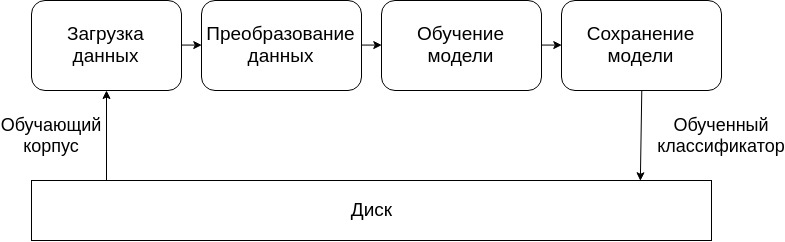
\includegraphics[width=.99\textwidth]{img/learn-module}
    \vspace*{6pt}
    \caption{Структура модуля обучения}\label{fig:project-tree}
  \end{figure}

 \

Для сохранения и загрузки файлов обученного классификатора была использована библиотека Joblib. \textbf{Joblib} — это набор инструментов для облегченной конвейерной обработки в Python. В частности, инструменты дампа и загрузки данных\cite{Joblib}.

Структура модуля обучения представлена на рисунке 2.2. Данный модуль с помощью описанных выше библиотек решает ряд задач: загрузку обучающих данных из файла, подготовку данных, извлечение признаков, нормализацию, построение и обучение классификатора, сохранение классификатора для дальнейшего использования. Этот модуль работает независимо от остальных модулей программы и используется только для создания обученной модели, поэтому взаимодействие с ним происходит с помощью интерфейса командной строки через интерпретатор Python. 

\newpage
\subsubsection{Проектирование модуля классификации}
\

Преобразование данных перед классификацией происходит так же, как и в обучающем модуле, посредством библиотеки Scikit-learn. Входными данными является текстовый документ, который необходимо классифицировать. Он представляется в виде вектора, после чего передается классификатору. Результатом классификации является метка класса, к которому относится входной документ, представленная в форме строки.

\

  \begin{figure}[h!]
    \centering
    \setlength{\fboxsep}{5pt}
    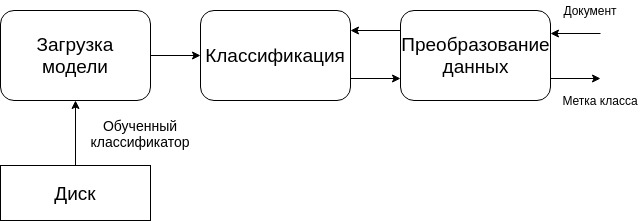
\includegraphics[width=.99\textwidth]{img/classification-module}
    \vspace*{6pt}
    \caption{Структура модуля обучения}\label{fig:project-tree}
  \end{figure}


Структура модуя классификации представлена на рисунке 2.3. Чтобы осуществить классификацию, необходимо сначала загрузить обученный классификатор и вспомогательные файлы (модели для преобразования входных данных) с диска. После загрузки модели классификатора с ним осуществляется взаимодействие с помощью интерфейса командной строки через интерпретатор Python или через модуль API.

\newpage
\subsubsection{Проектирование API}
\

Для соответствия программы нефункциональному требованию о возможности интеграции в другое приложение был разработан модуль API. Он представляет из себя веб-сервер, созданный с использованием Flask. \textbf{Flask} — фреймворк для создания веб-приложений на языке программирования Python, относится к категории микрофреймворков — минималистичных каркасов веб-приложений, предоставляющих лишь самые базовые возможности\cite{Flask}. Этот фреймворк в рамках данной работы был выбран для создания API из-за его минималистичности, простоты использования и запуска. 

Взаимодействие клиента с API произходит через HTTP-запросы. HTTP — протокол прикладного уровня передачи данных, в настоящий момент используется для передачи произвольных данных. Основой HTTP является технология «клиент-сервер», то есть предполагается существование:

\begin{itemize}
  \item Клиентов, которые инициируют соединение и посылают запрос;
  \item Серверов, которые ожидают соединения и запроса, производят необходимые действия и возвращают клиенту сообщение с результатом. 
\end{itemize}

Серверная часть API извлекает требующий классификации документ из запроса, передает его модулю классификации, и, получив ответ классификатора, возвращает этот ответ клиенту посредсвом HTTP.
\newpage
  \mysection{ОПИСАНИЕ ПРОЦЕССА РАЗРАБОТКИ ПРОГРАММЫ}
\

Программа прдставляет собой набор модулей на языке Python. Далее будет описан процесс разработки каждого из модулей программы.

\

\subsection{Модуль обучения}
\

Модуль обучения представлен классом на языке Python, который содержит метод для загрузки корпуса данных, метод, в котором происходит преобразование данных корпуса, построение и обучение модели, а также метод сохранения обученной модели на диск.

Для преобразования набора обучающих данных в массив векторов используется класс библиотеки Scikit-learn CountVectorizer. Он принимает в качестве аргумента конструктора разделитель, производит токенизацию всех документов коллекции, на этой основе составляет словарь токенов коллекции и конвертирует все документы в вектора, содержащие количество вхождений токена в каждый документ\cite{Scikit}.

\newpage 
  
\mysection{ТЕСТИРОВАНИЕ РАЗРАБОТАННОЙ ПРОГРАММЫ}
\

Тестирование — процесс исследования, испытания программного продукта, является одним из этапов разработки любого программного обеспечения. Оно необходимо для выявления ошибок во время разработки и после её завершения, проверки соответствия между ожидаемым поведением программного обеспечения и реальным, а также оценки качества программного обеспечения. Другими словами, тестирование — это одна из техник контроля качества программного продукта, включающая в себя действия по планированию работ (Test Management), проектированию тестов (Test Design), выполнению тестов (Test Execution) и анализу полученных результатов (Test Analysis).

Качество программного обеспечения (Software Quality) — это способность программного продукта удовлетворять предъявляемым к нему требованиям. 

Основные цели тестирования:

\begin{itemize}
	\item Повышение вероятности правильной работы при любых обстоятельствах.
	\item Повышение вероятности соответствия всем предъявленным к продукту требованиям.
	\item Предоставление актуальной информации о состоянии продукта на данный момент.
\end{itemize}

Для тестирования программы поиска был создан отдельный модуль.

\newpage

\subsection{Тестирование программы}
\

При тестирования программы использовалось модульное тестирование. Модульное тестирование — процесс, который позволяет проверить на корректность отдельные модули. Такое тестирование позволяет точно определить местонахождение ошибки, так как компоненты тестируются независимо друг от друга. Модульные тесты позволяют проверить, не привело ли очередное изменение кода к регрессии (появление ошибок в частях программы, которые уже были протестированы).

С помощью данного вида тестирования проверялись все методы разработанных классов, отражающие функционал сохранения, загрузки, выявления несуществующих названий моделей.

Также были протестированы некоторые неоднозначные случаи, в которых программа должна была повести себя определенным образом. Например, название модели конкурента может иметь пробел в середине, а название модели владельца магазина может быть написано слитно, или наоборот, но программа должна определить, что это одна и та же модель. Также было проверено соответствие функциональному требованию о том, что товары с несуществующими у владельца названиями моделей и идентификационными номерами не должны находиться.

\newpage

\subsection{Тестирование модели}
\

Под тестированием модели в данной работе подразумевается выявление её характеристик работы и проверка соответствия значений этих характеристик установленным ранее требованиям.

Скользящий контроль или кросс-проверка или кросс-валидация (cross-validation, CV) — процедура эмпирического оценивания обобщающей способности алгоритмов, обучаемых по прецедентам. 

Исходный набор данных разделяется на две подвыборки: обучающую и контрольную. Для каждого разбиения выполняется построение модели на основе обучающей подвыборки, затем оценивается её средняя ошибка на объектах контрольной подвыборки. Оценкой кросс-валидации называется средняя по всем разбиениям величина ошибки на контрольных подвыборках.

Скользящий контроль является стандартной методикой тестирования и сравнения алгоритмов классификации, регрессии и прогнозирования. 

С помощью кросс-валидации определялась точность предсказаний, из всего корпуса данных выделялось 20\% в качестве контрольной подвыборки, 80\% в качестве обучающей. Модель была обучена несколько раз на разном количестве документов в обучающей коллекции. При этом каждый раз замерялось и сохранялось время обучения. Далее для каждого случая модель классифицировала 100 разных документов и среднее время ответа было определено как время работы модели.

Результаты описанных выше действий представлены в таблице 4.1. На основании этих данных можно сделать следующие выводы:

\begin{itemize}
	\item Характеристики времени работы и точности классификации удовлетворяют заданным требованиям;
	\item Время обучения нелинейно растет при увеличении количества документов в корпусе данных;
	\item Характеристики точности и времени работы слабо варьируются для разного количества документов в рамках данного теста.
\end{itemize}

\begin{table}[h!]
\caption{Характеристики программы}
\label{props}
\centering
    \begin{tabular}{|c|c|c|c|}
		\hline Корпус, пар & Время обучения, с & Время работы, с & Точность, \% \\
		\hline 50000 & 384,1475 & 0.0003 & 96 \\
		\hline 20000 & 79.8404 & 0.0001 & 98 \\
		\hline 10000 & 11.7035 & 0.0001 & 98 \\
		\hline 5000 & 2.5664 & 0.0001 & 97 \\
		\hline 1000 & 0.3084 & 0.0001 & 98 \\
		\hline
	\end{tabular}
\end{table}
\

\newpage


  \mysection*{ЗАКЛЮЧЕНИЕ}

В рамках проведённой работы были получены следующие результаты:
\begin{dashitemize}
  \item 1.
  \item 2.
  \item 3.
\end{dashitemize}

\newpage

Автор планирует продолжать работу над проектом и~развивать его, добавляя новые функции и~исправляя возможные ошибки, которые могут быть найдены во время эксплуатации приложения.

\newpage

  \phantomsection
  \addcontentsline{toc}{section}{Библиографический список}

  \hyphenpenalty=10000
  \interlinepenalty=10000

  \nocite{*}
  \bibliography{build/all}
  
  \clearpage
  
  %\begin{appendices}
    %\input{src/appendices/events_module_listing}
    %\input{src/appendices/toggle_tests_listing}
  %\end{appendices}
\end{document}
